\documentclass[a4paper,11pt]{article}
\usepackage{setspace}
\onehalfspacing
 
\usepackage{titlesec}
\usepackage{graphicx}
\usepackage{listings}
\usepackage{xcolor}
\usepackage{fancyhdr}
\usepackage[a4paper,margin=1in]{geometry}
\usepackage{mdframed} %nice frames

\definecolor{light-gray}{gray}{0.95} %the shade of grey that stack exchange uses

\renewcommand{\thispagestyle}[1]{} % do nothing

\lstset{
  language=Python,
  aboveskip=3mm,
  belowskip=3mm,
  showstringspaces=true,
  columns=flexible,
  basicstyle={\small\ttfamily},
  numbers=none,
  numberstyle=\tiny\color{gray},
  keywordstyle=\color{blue},
  commentstyle=\color{red},
  breaklines=true,
  breakatwhitespace=true,
  tabsize=2
}

\graphicspath{ {./images/} }
\titlespacing{\section}{0pc}{1pc}{1pc}
 
\pagestyle{fancy}
\fancyhf{}
\rhead{Assignment 3}
\lhead{Design \& Implementation: Internet Voice \& Text Chatting Program}
\rfoot{Page \thepage}

 
\begin{document}
\title{\vspace{-1.0cm}\textbf{Design \& Implemenation: \linebreak Internet Voice \& Text Chatting Program}}
\author{
  \textbf{Tan Wei Xuan (49003140)}\\
  \texttt{tanweixuan@postech.ac.kr}
  \and
   \textbf{Zhang Xin Yue (49003143)}\\
  \texttt{xyzhang@postech.ac.kr}
}
\date{\today}
\maketitle

\section{Project Overview}
The\textbf{ Internet Text and Voice Messaging Program} that I have implemented is a \textbf{Multi-threaded Chat Application} that utilises the Transmission Control Protocol \textit{(TCP)} and allows for mutiple clients to send/receive text and voice messages over a server, to one another, at the same time.  We switched from using \textit{Java} to \textit{Python} as \textit{Python} provides more API support for voice chat. The source code files are as follow:
\begin{enumerate}
	\item \textbf{Server Files}
\begin{itemize}
  	\item server.py
\end{itemize}
	\item \textbf{Client Files}
\begin{itemize}
  	\item client.py
\end{itemize}
\end{enumerate}

\section{Environment and Dependencies}
My program is written in \textbf{Python 3.6.7} and is developed on \textbf{Windows running the Ubuntu 18.04.2 bit subsystem}, using \textbf{PyCharm} as the \textbf{Integrated Development Environment}. \textit{The program may not work as inteneded if it is ran on other environments.}
\textit{\textbf{Ensure that these dependencies are being installed on your system}}.
\begin{enumerate}
  \item \textbf{PyAudio}
\begin{mdframed}[backgroundcolor=light-gray, roundcorner=30pt,leftmargin=1, rightmargin=1, innerleftmargin=5, innertopmargin=-3,innerbottommargin=5, outerlinewidth=1, linecolor=light-gray]
\begin{lstlisting}
#On Ubuntu Terminal
$ sudo apt-get install python-pyaudio python3-pyaudio
\end{lstlisting}
\end{mdframed}
  \item \textbf{Threading}
\begin{mdframed}[backgroundcolor=light-gray, roundcorner=30pt,leftmargin=1, rightmargin=1, innerleftmargin=5, innertopmargin=-3,innerbottommargin=5, outerlinewidth=1, linecolor=light-gray]
\begin{lstlisting}
#On Ubuntu Terminal
$ sudo apt install python3-pip #Only if pip is not installed
$ pip install threaded
\end{lstlisting}
\end{mdframed}
  \item \textbf{libasound}
\begin{mdframed}[backgroundcolor=light-gray, roundcorner=30pt,leftmargin=1, rightmargin=1, innerleftmargin=5, innertopmargin=-3,innerbottommargin=5, outerlinewidth=1, linecolor=light-gray]
\begin{lstlisting}
#On Ubuntu Terminal
$ sudo apt-get install libasound2-devf
\end{lstlisting}
\end{mdframed}
\end{enumerate}

\section{Implementation - Text Chat}

\subsection{Client - Receving Text }
Below is the handler for how a client receives text sent from other clients through the server. The Client is binded to the Server Text Port on \textit{2222}.
\begin{mdframed}[backgroundcolor=light-gray, roundcorner=30pt,leftmargin=1, rightmargin=1, innerleftmargin=5, innertopmargin=-3,innerbottommargin=5, outerlinewidth=1, linecolor=light-gray]
\begin{lstlisting}
#Client.py
def receive_text():
	while True:
		try:
			msg = client_socket_text.recv(BUFSIZ).decode("utf8")
			print(msg)
		except OSError:
			break
\end{lstlisting}
\end{mdframed}

\subsection{Client - Sending Text}
Below is the handler for how a client sent a text to the server and to other clients on the server. The Text and Video Port connection will be closed if the Client inputs \textit{"quit"}.
\begin{mdframed}[backgroundcolor=light-gray, roundcorner=30pt,leftmargin=1, rightmargin=1, innerleftmargin=5, innertopmargin=-3,innerbottommargin=5, outerlinewidth=1, linecolor=light-gray]
\begin{lstlisting}
#Client.py
def send_text():
	while True:
		msg = input()
		print('\033[A\033[A')
		client_socket_text.send(bytes(msg, "utf8"))
		if msg == "{quit}":
			client_socket_text.close()
			client_socket_voice.close()
			quit()
\end{lstlisting}
\end{mdframed}

\subsection{Server - Accept Connection to Text Port}
Below is the handler for how the server accepts a connection from the client onto the Text Port. The Text Port that the client connect to is \textit{2222}. Whenever a client is connected to the port, a thread if attached to the client to handle it.
\begin{mdframed}[backgroundcolor=light-gray, roundcorner=30pt,leftmargin=1, rightmargin=1, innerleftmargin=5, innertopmargin=-3,innerbottommargin=5, outerlinewidth=1, linecolor=light-gray]
\begin{lstlisting}
#Server.py
#For handling client's connection to TEXT PORT, assign a thread for each connection
def accept_text():
	while True:
		client, client_address = SERVER_TEXT.accept()
		print("%s:%s has connected from ." % client_address)
		client.send(bytes("Enter your name: ", "utf8"))
		addresses_text[client] = client_address
		Thread(target=handle_client_text, args=(client,)).start()

\end{lstlisting}
\end{mdframed}

\subsection{Server - Handling Text}
Below is the handler for how the Server recevies a message from a client and subsequently broadcasts the message to all the other clients on the server.
\begin{mdframed}[backgroundcolor=light-gray, roundcorner=30pt,leftmargin=1, rightmargin=1, innerleftmargin=5, innertopmargin=-3,innerbottommargin=5, outerlinewidth=1, linecolor=light-gray]
\begin{lstlisting}
#Server.py
def handle_client_text(client):
  #Handles a message from the given socket.
	#Receive Message
	name = client.recv(BUFSIZ).decode("utf8")
	welcome = 'Welcome %s! Type {quit} to exit the chat room.' % name
	client.send(bytes(welcome, "utf8"))
	msg = "%s has entered the chat room!" % name
	broadcast(bytes(msg, "utf8"))
	clients_text[client] = name

	while True:
		msg = client.recv(BUFSIZ)
		if msg != bytes("{quit}", "utf8"):
			#Append name to front of message
			broadcast(msg, name + ">> ")
		else:
			client.send(bytes("{quit}", "utf8"))
			client.close()
			erase_client(client)
			broadcast(bytes("%s has left the chat room." % name, "utf8"))
			break

\end{lstlisting}
\end{mdframed}


\section{Implementation - Voice Chat}
We utlisied the PyAudio library to implement the voice chat portion of our application.

\subsection{Client - Declaring the Input/Output Streams}
We have to declare the Input and Output Stream for sending and receiving audio on our client. \textit{stream send} is for sending our voice input to the server, on onto the other clients on the server. \textit{stream receive} is for receving and playing the voice output from the server, which is sent from the other clients on the server.
\begin{mdframed}[backgroundcolor=light-gray, roundcorner=30pt,leftmargin=1, rightmargin=1, innerleftmargin=5, innertopmargin=-3,innerbottommargin=5, outerlinewidth=1, linecolor=light-gray]
\begin{lstlisting}
#Client.py
#For sending stream over to the server
stream_send = p.open(
	format=pyaudio.paInt16,
	channels=CHANNELS,
	rate=RATE,
	input=True,
	frames_per_buffer=CHUNK)

#For receving stream from the server and playing the stream
stream_recv = p.open(
	format=p.get_format_from_width(WIDTH),
	channels=CHANNELS,
	rate=RATE,
	output=True,
	frames_per_buffer=CHUNK)

\end{lstlisting}
\end{mdframed}

\subsection{Client - Sending/Receiving  Audio}
The client have to handles both sending/receiving voice simulatanuously. The below two functions are for receiving and playing the voice sent from the server and for sending voice inputs from the client to the server. The Client is binded to the Server Voice Port on \textit{55555}.
\begin{mdframed}[backgroundcolor=light-gray, roundcorner=30pt,leftmargin=1, rightmargin=1, innerleftmargin=5, innertopmargin=-3,innerbottommargin=5, outerlinewidth=1, linecolor=light-gray]
\begin{lstlisting}
#Client.py

# For Receiving Voice
def receive_voice():
	while True:
		try:
			data = client_socket_voice.recv(BUFSIZ)
			stream_recv.write(data)
		except OSError:
			break

# Send voice to the server
def send_voice():
	while True:
		try:
			data = stream_send.read(CHUNK)
			client_socket_voice.sendall(data)
		except OSError:
			break
clientSocket.close();
\end{lstlisting}
\end{mdframed}

\subsection{Server - Accept Connection to Voice Port}
Below is the handler for how the server accepts a connection from the client onto the Voice Port. The Voice Port that the client connect to is \textit{55555}. Whenever a client is connected to the port, a thread if attached to the client to handle it.

\begin{mdframed}[backgroundcolor=light-gray, roundcorner=30pt,leftmargin=1, rightmargin=1, innerleftmargin=5, innertopmargin=-3,innerbottommargin=5, outerlinewidth=1, linecolor=light-gray]
\begin{lstlisting}
#Server.py
 For handling client's connection to VOICE PORT, assign a thread for each connection
def accept_voice():
	while True:
		client, client_address = SERVER_VOICE.accept()
		addresses_voice[client] = client_address
		Thread(target=handle_client_voice, args=(client,)).start()
\end{lstlisting}
\end{mdframed}


\subsection{Server - Handling Voice}
Below is the handler for how the Server recevies a voice message from a client and subsequently broadcasts the message to all the other clients on the server.
\begin{mdframed}[backgroundcolor=light-gray, roundcorner=30pt,leftmargin=1, rightmargin=1, innerleftmargin=5, innertopmargin=-3,innerbottommargin=5, outerlinewidth=1, linecolor=light-gray]
\begin{lstlisting}
#Server.py
def handle_client_voice(client):
	"""
	Handles Voice from the given socket.
 	"""
	# Receive Voice
	clients_voice[client] = 1

	while client in clients_voice:
		try:
			data = client.recv(BUFSIZ)
			broadcast(data, dtype='voice')
		except Exception as _:
			client.close()
			del clients_voice[client]

\end{lstlisting}
\end{mdframed}

\section{Running the Program}
\textit{On the client, the input for host should be \textbf{127.0.0.1} unless a specific host has been defined.}
\subsection{Terminal}
\begin{enumerate}
  \item In the terminal, run the command \textbf{\textit{python Server.py}} to start the \textbf{server}.
  \newline
  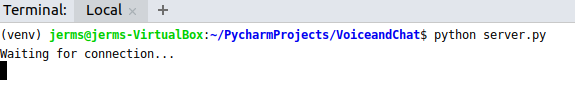
\includegraphics{server}
  \item In the terminal, run the command \textbf{\textit{python Client.py}} to start the \textbf{client}. (Run \textit{\textbf{n}} times to start \textit{\textbf{n}} clients)
  \newline
  \includegraphics{client}
   \item Voice is constantly is being sent \& received, so you do not have to input any additional commands to enable voice chat. 
   \item In the terminal, type \textbf{\{quit\}} to exit the from the server.
   \newline
   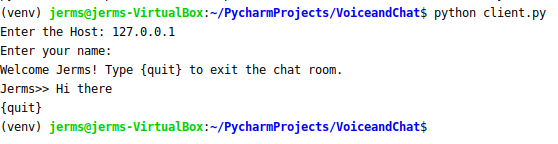
\includegraphics{exit}
\end{enumerate}

\section{Limitations}
Our Program is executed on a single machine running multiple clients, that is the machine is the host of the server as well as the host for all the clients. The voice feedback (echo) as heard from \textit{Screen Record of Program Execution.mp4} signifies that the voice has been received and played from one client to another. Future improvements can bbe made to allow the server and clients to run on seperate machines.

\end{document}